\documentclass{scrartcl}

\usepackage{graphicx}
\usepackage[utf8]{inputenc}
\usepackage[T1]{fontenc}
\usepackage{lmodern}
\usepackage{babel}
\usepackage{amsmath}
\usepackage{amsthm}
\usepackage{mathtools}
\usepackage{amssymb}
\usepackage{listings}
\usepackage{xparse}
\usepackage{geometry}
\usepackage{enumerate}
\usepackage{tikz}
\usepackage[style=english]{csquotes}
\usepackage[language=english, backend=biber, style=alphabetic, sorting=nyt]{biblatex}

\usetikzlibrary{babel, positioning, shapes.geometric, arrows, arrows.meta}
\addbibresource{bibliography.bib}

\title{The Supersingular Diffie-Hellmann Key Exchange protocol}
\author{Simon Pohmann}

\newcommand{\N}{\mathbb{N}}
\newcommand{\Z}{\mathbb{Z}}
\newcommand{\F}{\mathbb{F}}
\newcommand{\aff}{\mathrm{aff}}
\renewcommand{\O}{O}

\newtheorem{prop}{Proposition}[section]
\newtheorem{theorem}[prop]{Theorem}
\newtheorem{alg}[prop]{Algorithm}
\newtheorem{definition}[prop]{Definition}
\newtheorem{example}[prop]{Example}
\newtheorem{remark}[prop]{Remark}

\begin{document}

\maketitle

\tableofcontents

\section{Elliptic Curves}

\subsection{The projective point of view}

\begin{definition}
    A (possibly nonsmooth) elliptic curve $E$ defined over a field $K$ is the (projective) zero set
    \begin{equation*}
        E = \{ (x : y : 1) \ | \ y^2 + a_1 xy + a_3 y = x^3 + a_2 x^2 + a_4 x + a_6 \} \cup \{ \O \} \subseteq \mathbb{P}_{\bar{K}}^2
    \end{equation*}
    of some irreducible polynomial $F(x, y) = y^2 + a_1 xy + a_3 y - x^3 - a_2 x^2 - a_4 x - a_6 \in K[x, y]$. 
    This equation is called a Weierstraß equation defining $E$.
    The point $\O := (0 : 1 : 0)$ here is the point at infinity of the elliptic curve.
\end{definition}

\begin{definition}
    \label{def:discriminant}
    A (possibly nonsmooth) elliptic curve $E$ defined by $y^2 + a_1 xy + a_3 y = x^3 + a_2 x^2 + a_4 x + a_6$ is called smooth, if the discriminant
    \begin{align*}
        \Delta(E) = & - b_2^2 b_8 - 8 b_4^3 - 27 b_6^2 + 9 b_2 b_4 b_6 \\
        \text{where} \ & b_2 = a_1^2 + 4 a_2 \\
        & b_4 = a_1 a_3 + 2 a_4 \\
        & b_6 = a_3^2 + 4 a_6 \\
        & b_8 = a_1^2 a_6 + 4 a_2 a_6 - a_1 a_3 a_4 + a_2 a_3^2 - a_4
    \end{align*}
    is nonzero. In this work, the term ``elliptic curve'' will be used for smooth elliptic curves.
\end{definition}

As elliptic curves are given as the zero set (or locus) of a polynomial, they are algebraic varieties and many properties can be studied using Algebraic Geometry.
In the more general context of Algebraic Geometry, an elliptic curve is usually defined as a smooth projective curve of genus 1.
As shown in \cite[III Prop 3.1]{arithmetic_elliptic_curves}, each elliptic curve by this definition is isomorphic to an elliptic curve defined by a Weierstraß equation.
Here ``isomorphic'' refers to $K$-variety isomorphisms in the sense of Algebraic Geometry.
As this is a fundamental notion, we will state the required special case here.

\begin{definition}
    For a (projective) algebraic variety $V \subseteq \mathbb{P}_{\bar{K}}^2$ given as the zero set of an ideal $I \leq K[x, y, z]$, its (projective) coordinate ring is given as $K[V] := K[x, y, z] / I$.
\end{definition}

\begin{definition}
    Given irreducible varieties $V, W \subseteq \mathbb{P}_{\bar{K}}^2$, a partial map $\phi: V \to W$ is called rational if it is given by rational functions.
    Namely, $\phi$ is rational if there are homogeneous $f_1, f_2, f_3 \in \bar{K}[V]$ of same degree and not all zero such that for each point $(x : y : z)$ at which $\phi$ is defined, there are ``equivalent'' polynomials $(g_1, g_2, g_3) \in \bar{K}[V], \ (g_1, g_2, g_3) \sim (f_1, f_2, f_3)$ such that
    \begin{equation*}
        (g_1(x, y, z) : g_2(x, y, z) : g_3(x, y, z)) \ \text{is nonzero and equal to $\phi(x : y : z)$}
    \end{equation*}
    Here we define equivalence as $(f_1, f_2, f_3) \sim (g_1, g_2, g_3)$ if $f_i g_j = f_j g_i$ for all $i, j$.
    We use the notation $\phi = [f_1, f_2, f_3]$.
\end{definition}

This definition is quite technical, as for well-definedness, we require that no denominator polynomial evaluates to 0 and do not get the projective (non-)point $(0 : 0 : 0)$. 

The intuition is that each component of a rational map is given by a quotient of polynomials.
If we want to evaluate the map at a point where the quotient is not well-defined, then we are allowed to ``fix'' it by dividing out a corresponding polynomial factor from all components.
This dividing out of a corresponding polynomial factor does not change the ratio of two homogeneous components, hence it does not change the projective point.
As $\bar{K}[V]$ is not a UFD, defining this division is not straightforward. 
Instead, we define a tuple of polynomials as equivalent, if the ratio of different components is the same in the coordinate ring.
Now equivalent polynomial tuples can be obtained from each other by some kind of ``abstract'' division.

\begin{definition}
    A rational map between varieties that is defined everywhere is called morphism. If it is bijective and its inverse is a morphism, it is called isomorphism.
\end{definition}

In the case of elliptic curves, things are easier than that. For example, if the domain is a smooth (elliptic) curve, then each rational map is a morphism (see \cite[II Prop 2.1]{arithmetic_elliptic_curves}).

\subsection{The affine point of view}

Because of many reasons, projective geometry is the ``correct'' way to describe varieties, hence elliptic curves are usually defined as projective curves.
In particular, most of Algebraic Geometry is done in projective space, and thus one may use the very powerful theory developed in this context.
For readers that are not used to projective geometry, one can use the embedding of the affine space $\bar{K}^2 \subseteq \mathbb{P}_{\bar{K}}^2$ via $(x, y) \mapsto (x : y : 1)$ to give an easier formulation that only works for elliptic curves.

\begin{remark}
    A (possibly nonsmooth) elliptic curve $E$ defined over a field $K$ is the affine zero set
    \begin{equation*}
        \{ (x, y) \in \bar{K}^2 \ | \ y^2 + a_1 xy + a_3 y = x^3 + a_2 x^2 + a_4 x + a_6 \} \subseteq \bar{K}^2
    \end{equation*}
    of some irreducible polynomial $F(x, y) = y^2 + a_1 xy + a_3 y - x^3 - a_2 x^2 - a_4 x - a_6 \in K[x, y]$ together with a point at infinity $\O := \infty$. 
\end{remark}

\begin{remark}
    A (possibly nonsmooth) elliptic curve $E$ is called smooth, if its discriminant $\Delta(E)$ (see \ref{def:discriminant}) is nonzero. In this work, the term ``elliptic curve'' will be used for smooth elliptic curves.
\end{remark}

Now we come to rational maps and morphisms. First, we require the affine coordinate ring of an elliptic curve.

\begin{definition}
    The affine coordinate ring of an elliptic curve defined by $F(x, y) := y^2 + a_1 xy + a_3 y - x^3 - a_2 x^2 - a_4 x - a_6 = 0$ is given as $K[E]_\aff := K[x, y] / (F(x, y))$.
\end{definition}

Note that we may evaluate elements $f \in K[E]_\aff$ at points $(x, y) \in E$, as each representative in the equivalence class will evaluate to the same value at $(x, y)$.

Now we want to define a rational map, but encounter some problems.
In particular, here we see a reason why the projective space is better suited for the study of elliptic curves, as the definition of rational maps using only the affine space is quite complicated and unsatisfying.
As one might expect, rational maps are maps whose components are given by fractions of polynomials (or more precisely, fractions of elements of the affine coordinate ring $K[E]_\aff$).
Problems now arise when considering points at which the denominator polynomial has a root.
In the only case that interests us, namely if the domain of the map is a smooth elliptic curve, there are two possibilities:

Sometimes, one can find another representative of the fraction in the quotient field of $K[E]_\aff$ where this problem no longer exists.
In this case, everything is well.

However, it can happen that no such representative exists. In this case, we will always find a representative, in which at least one of the numerators of the components evaluate to a nonzero value.
In this component, we conceptually have a $\frac 1 0 = \infty$, so will get a point at infinity. However, these points at infinity are not contained in the affine space and thus we cannot describe them sufficiently.
In the case of elliptic curves, there is only one point at infinity (namely $\O$), so this might be possible in theory. 
However, the resulting definition would be cluttered case distinctions and highly non-instructive.

Here, we settle now for a moderately simple description of rational maps $\phi: E \to E'$ between elliptic curves that describes their behavior everywhere except at $\O$.
Most importantly, this will suffice to define isogenies later.

\begin{remark}
    A rational map $\phi: E \to E'$ between elliptic curves fulfills the following condition:
    Either $\phi = \O$ is constant or there are elements $f_1, f_2, g \in \bar{K}[E]_\aff, g \neq 0$ such that for all points $(x, y) \in \bar{K}^2$ at which $\phi$ is defined, there are $f_1', f_2', g' \in K[E]_\aff, g' \neq 0$ with
    \begin{align*}
        \left(\frac {f_1'} {g'}, \frac {f_2'} {g'}\right) = \left(\frac {f_1} g, \frac {f_2} g\right) \ &\text{in the field of fractions of $K[E]_\aff$ and} \\
        \left(\frac {f_1'(x, y)} {g'(x, y)}, \frac {f_2'(x, y)} {g'(x, y)}\right) \ &\text{is defined and equal to $\phi(x, y)$}
    \end{align*}
    Here we say that only $(\frac 0 0, \frac 0 0)$ is not defined, and let $(\frac a 0, \frac b 0) := \O = \infty$ for $(a, b) \neq (0, 0)$.
    We use the notation $\phi = [f_1, f_2, g]$.
\end{remark}

This description is almost a complete definition, in the sense that a map $\phi$ is rational if and only if its behavior on $\bar{K}^2$ is given by $\phi = [f_1, f_2, g]$ as above and the value $\phi(\O)$ is equal to the value at infinity one can define for $f_1, f_2, g$.

\subsection{Simpler formulas}

The general Weierstraß equation is still relatively complicated. If the characteristic of $K$ is not $2$ or $3$ however, we have the following simpler representation:

\begin{prop}
    Let $E$ be an elliptic curve defined over $K$ by the Weierstraß equation $y^2 + a_1 xy + a_3 y = x^3 + a_2 x^2 + a_4 x + a_6$.
    Then $E$ is isomorphic to an elliptic curve defined by a Weierstraß equation of the form
    \begin{equation*}
        y^2 = x^3 - Ax - B
    \end{equation*}
    where $A, B \in K$. Here ``isomorphic'' means $K$-variety isomorphic (in the sense of Algebraic geometry).
\end{prop}

\section{Isogenies}

\begin{prop}
    \label{prop:unique_isogeny}
\end{prop}

\begin{prop}
    \label{prop:velu_formulas}
\end{prop}

\section{Supersingular Diffie-Hellmann}

\subsection{The Key Exchange}
Consider the following key exchange protocol:
\begin{description}
    \item[Public data] 
        Choose primes $l_A, l_B$ such that $p := l_A^{e_A} l_B^{e_B} f \pm 1$ is prime for some (small) $f \in \N$. Now find a supersingular elliptic curve $E$ defined over $\F_q$ with $q = p^2$ and
        \begin{equation*}
            E(\F_q) \cong \left( \Z / (p \mp 1) \Z \right)^2
        \end{equation*}
        In particular, every subgroup is a free rank 2 $\Z$-module, and so we find a basis $P_A, Q_A$ of the $l_A^{e_A}$-torsion subgroup $E[l_A^{e_A}]$ of $E(\F_q)$ and similarly $P_B, Q_B$ of $E[l_B^{e_A}]$.
        \begin{center}
            The public data consists now of $l_A, e_A, l_B, e_B, E, P_A, Q_A, P_B, Q_B$
        \end{center}
    \item[Secret Generation] 
        Alice chooses a secret point $A := [m_A]P_A + [n_A]Q_A \in E[l_A^{e_A}]$ with maximal order $l_A^{e_A}$ using random $m_A, n_A \in \Z$. 
        Similarly, Bob chooses a secret point $B := [m_B]P_B + [n_B]Q_B \in E[l_B^{e_B}]$ with maximal order $l_B^{e_B}$. Note that these points correspond to unique separable isogenies
        \begin{equation*}
            \alpha: E \to E_A \ \text{and} \ \beta: E \to E_B
        \end{equation*}
        with kernels $\langle A \rangle$ resp. $\langle B \rangle$. 
        Now they publish $E_A$ and $E_B$ and additionally $\alpha(P_B), \alpha(Q_B)$ resp. $\beta(P_A), \beta(Q_A)$.
        \begin{center}
            Secret are $m_A, n_A, m_B, n_B$ resp. $A, B, \alpha, \beta$; \\
            Public are $E_A, E_B, \alpha(P_B), \alpha(Q_B), \beta(P_A), \beta(Q_A)$
        \end{center}
    \item[Key Computation]
        Alice now computes $A' := [m_A]\beta(P_A) + [n_A]\beta(Q_A) \in E_B(\F_q)$ and the unique separable isogeny
        \begin{equation*}
            \alpha': E_B \to E_{BA}
        \end{equation*}
        with kernel $\langle A' \rangle$. 
        Similarly, Bob computes $B' := [m_B]\alpha(P_B) + [n_B]\alpha(Q_B)$ and the unique separable isogeny
        \begin{equation*}
            \beta': E_A \to E_{AB}
        \end{equation*}
        with kernel $\langle B' \rangle$. 
        \begin{center}
            Now have the joint key $j(E_{AB}) = j(E_{BA})$
        \end{center}
\end{description}
Note $l_A^{e_A}l_B^{e_B}f \pm 1$ is prime relatively often, so in the first step, we can simply try multiple choices and use a suitable one.
The isogeny computations can be efficiently done using Velu's formulas (\ref{prop:velu_formulas}).
To show correctness, it suffices now to show that $j(E_{AB}) = j(E_{BA})$.
\begin{proof}
    As $B' = \alpha(B)$ have $\alpha^{-1}(\{B'\}) = \ker(\alpha) + B = \langle A \rangle + B$.
    Hence
    \begin{equation*}
        \ker(\beta' \circ \alpha) = \alpha^{-1}(\ker(\beta')) = \alpha^{-1}(\langle B' \rangle) = \langle A + \langle B \rangle \rangle = \langle A, B \rangle
    \end{equation*}
    Similarly get that $\ker(\alpha' \circ \beta) = \langle A, B \rangle$. Now \ref{prop:unique_isogeny} yields that $E_{AB} \cong E_{BA}$ and thus they have the same j-invariant.
    Up to isomorphism, this is shown by the following commutative diagram:
    \begin{center}
        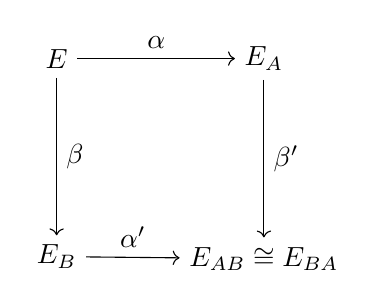
\begin{tikzpicture}[node distance = 2cm]
            \node (E) {$E$};
            \node (EA) [right = of E] {$E_A$};
            \node (EB) [below = of E] {$E_B$};
            \node (EAB) [below = of EA] {$E_{AB} \cong E_{BA}$};
            \draw [->] (E) -- node [above, midway] {$\alpha$} (EA);
            \draw [->] (E) -- node [right, midway] {$\beta$} (EB);
            \draw [->] (EA) -- node [right, midway] {$\beta'$} (EAB);
            \draw [->] (EB) -- node [above, midway] {$\alpha'$} (EAB);
        \end{tikzpicture}
    \end{center}
\end{proof}

\printbibliography

\end{document}